\documentclass[a4paper,11pt]{article}
\usepackage{geometry}
\usepackage[T1]{fontenc}
\usepackage{apacite}
\usepackage{graphicx}
% \usepackage{natbib}
\usepackage{adjustbox}
\bibliographystyle{apacite}
\usepackage{xurl}
\urlstyle{same}
\geometry{a4paper, margin=3cm}

\begin{document}


\begin{titlepage}
    \centering
    \vspace*{2cm}
    
    \textbf{\Large Research report}
    
    \vspace{2cm}
    
    \textbf{\Huge Enhancing Causal Inference with Network Information}
    
    \vfill
    
    \textbf{Polina Revina (8461465)}
    
    \vspace{0.5cm}
    
    \textbf{Supervisors: Erik-Jan van Kesteren, Javier Garcia-Bernardo}
    
    \vspace{0.5cm}
    
    \textit{Methodology and Statistics for the Behavioural, Biomedical and Social Sciences\\
    Utrecht University}
    
    \vfill
    \textbf{\today}
    \vspace{0.5cm}
    
    \textbf{Word count: 1863}
    \vspace{0.5cm}
    
    Candidate journals: Statistical Science; Sociological Methods \& Research \\ 
    
\end{titlepage}
\nocite{*}

\section{Introduction}
In many experimental and observational studies, network interference is present between units, which means that the treatment of one unit affects the results of its neighbors \cite{cox1958planning}. This happens because of transmission of exposure through social interaction or physical proximity of units. For example, students who received tutoring support can interact with other students not assigned to this program and transmit the knowledge obtained during tutoring \cite{forastiere2021identification}. Another example is vaccine trials on infectious diseases, when treated individuals can affect the likelihood of disease transmission and influence the infection rate.

The assumption of no interference lies at the heart of causal inference, forming a fundamental component of the Stable Under Treatment Value Assumption \cite{rubin1974estimating}. As demonstrated by Sobel \citeyear{sobel2006randomized}, using methods that do not account for interference or imposing this assumption incorrectly can lead to an entirely wrong conclusion about the effect. This complicates causal estimations in settings with interdependent units, such as social networks, communities, or economic systems.

Addressing the issue of interference led to the development of two primary types of strategies: design strategies that focus on mitigating interference in experiments and inference strategies that use network data to adjust estimations. The widely used approach for estimation in these settings is to relax the no interference assumption by localizing interference within certain structures or defining its form. Under partial interference, units within each cluster can affect each other's outcome, but between clusters, no interference occurs \cite{sobel2006randomized}. This assumption is often used with stratified interference, where the level of interference depends on the proportion of treated units within the group \cite{savje2021average}. This framework provides a foundation for the development of experimental designs, such as cluster-based randomization and its extensions such as two-stage randomization \cite{hudgens2008toward}, graph cluster randomization \cite{ugander2013graph}.

Recent studies focused on relaxing the partial interference assumption, allowing units to interfere along more general structures, such as social networks \cite{manski2013identification}, but suggested estimation methods require knowledge of the interference structure. To overcome this shortage, Savje et al. \citeyear{savje2021average} proposed a new estimand Expected Average Treatment Effect (EATE), which marginalizes the unit-level treatment effect over all possible reference assignments, capturing the average treatment effect while accounting for interference. The proposed estimand shows consistency under weak interference assumption without knowledge of the interference structure.

However, these assumptions about interference are rarely likely to hold, especially in high-dimensional networks, so another approach uses new estimators to adjust for network information. Forastiere et al. \citeyear{forastiere2021identification} propose a generalized propensity score method that adjusts for network information by balancing individual and neighborhood covariates. This method aims to reduce confounding by estimating the probabilities of treatment assignment while accounting for the relationships between individuals in the network. Another significant contribution is the extension of the Targeted Maximum Likelihood Estimator, enabling it to handle situations where the treatment effect is influenced by spillovers from neighboring units \cite{ogburn2024causal}.

Recent studies utilize modern developments of neural networks to adjust inference. Leung et al. \citeyear{leung2022graph} used graph neural networks (GNN), a powerful method to capture complex dependencies in the graph to estimate the direct effect under interference. Khatami et al, \citeyear{khatami2024graph} combined GNN with double machine learning framework for unbiased and efficient estimations, thus providing valid confidence intervals.

\subsection{Research question}
There is still a limited understanding of the degree of bias of causal inference estimators in observational studies under different exposure scenarios and network structures. Current studies are more focused on experimental design than observational studies and often rely on the partial interference assumption, which may not reflect more complex scenarios where interference can occur across groups. Existing methods for network adjustment also lack a theoretical base and their application in observational studies is limited. 

This project aims to enhance causal inference methods for observational data by incorporating network information. The research question is \textit{"To what extent does network interference produce bias in standard causal inference estimates and how can network properties be used to reduce the bias?"}

\section{Data}
For the analysis, I generated synthetic data to simulate how both the outcome and treatment spread through the network, reflecting the underlying structure and interactions. By controlling for relevant variables, estimation bias from not accounting for network interference can be estimated. The key parameters in the data generation process are summarized in Table~\ref{tab:parameters}.

\begin{table}[h!]
\centering
\begin{tabular}{|l|l|}
\hline
\textbf{Parameter}         & \textbf{Description}                                                                               \\ 
\hline
Network Models             & Barabási-Albert, Watts-Strogatz, Erdős-Rényi (10,000 nodes each)                                       \\ \hline
Neighbor Influence         & Small (0.1), Medium (0.3), Large (0.7)                                                                 \\ \hline
Covariate                & \(N(5, 20)\)                              \\ \hline
Treatment effect        & Medium (0.3)                                                                 \\ \hline
\end{tabular}
\caption{Key parameters and descriptions used in the data generation process.}
\label{tab:parameters}
\end{table}


\subsection{Treatment assignment}
I assume a simple contagion, meaning that one connection to the treated is enough for the effect transmission \cite{cencetti2023distinguishing}. One of the features of this mechanism is that the rate of adoption is proportional to the number of exposures, so being in contact with two treated individuals doubles the overall rate. The assignment of treatment is random, and the split between control and treatment groups is equal. For the first simulation the medium effect (30\%) is used. 

\subsection{Network generation}

Different types of networks are used in this research to account for various phenomena. This allows us to capture a range of scenarios, such as friends groups, social media websites or purely random interaction. Moreover, as it remains unclear whether and how the type of network structure influences the estimation bias of network interference, it is essential to explore different models. For every network model, ten thousand nodes are generated. The generated network will be represented as an adjacency matrix, denoted $W$, which encodes the connections between nodes and serves as the foundation for further analysis.

The \textit{\textbf{Barabási-Albert model}} is well suited to simulating real-world systems that exhibit scale-free properties, such as friendship groups, high school social networks, or online platforms, where a small number of nodes tend to accumulate a disproportionately large number of connections \cite{bertotti2019configuration}. 

In addition, the \textit{\textbf{Watts-Strogatz model}} is generated to create small-world networks, characterized by high clustering and short average path lengths, features commonly observed in many social and biological systems. This model is useful for studying phenomena like information diffusion or community formation, as it captures the balance between local and global connectivity within a network \cite{song2014simple}.

The \textit{\textbf{Erdős-Rényi model}} generates random networks in which each possible edge between nodes has a fixed probability. This model is often used as a benchmark to understand how randomness alone can shape network structures and dynamics. While it lacks the clustering seen in the Watts-Strogatz model or the hubs in the Barabási-Albert model, it provides a baseline for comparison by modelling purely stochastic connections.

\subsection{Covariate}
Covariate represents individual-level characteristics, such as age or income. They are generated from a normal distribution $N(5, 20)$, its distribution does not have a theoretical foundation and is used only for data generation. 

\subsection{Outcome}
The outcomes in the network will be simulated using a \textbf{spatial autocorrelation model} (SAR), which accounts for the dependencies incorporated in the network structure. This model captures how an individual’s outcome is influenced by their neighbours' responses, individual-level covariates, and independent noise. 

A key assumption of the SAR model is indirect interference, which implies that spillovers are proportional to the effect of direct treatment. That is, if there is no direct effect of treatment on a unit, there will be no spillovers to its neighbours. This assumption is integral to the linearity of the model and serves as a foundation for simulating outcomes in networks.

Formally, the outcome can be expressed as: $y = (I - \rho W)^{-1} X\beta + (I - \rho W)^{-1} \epsilon$, where $\rho$ represents the influence of neighbors, $\W$ is the adjacency matrix capturing network connections, $X$ is a matrix of covariates, and $\epsilon$ represents independent noise. 

The coefficients $\beta$ are sampled from a normal distribution $N(3, 10)$, and the neighbour influence parameter $\rho$ will take on values corresponding to small (0.1), medium (0.3), and large (0.7) levels of spillover intensity. This approach allows us to model varying degrees of dependence between connected individuals and analyze the propagation of treatment effects through the network.

\section{Methods}
\subsection{Linear regression}
In this context, the estimand of interest is the Average Treatment Effect (ATE), which captures the average difference in outcomes between the treatment and control groups. The ATE provides a measure of the impact of the treatment assignment in the population when SUTVA holds.

As treatment is assigned randomly, to estimate effect I used the following linear regression: $y = \beta_0 + \beta_1*Covariate_{i} + \beta_2*Group_{i} + \epsilon_{i}$, where $Group_i$ indicates individuals' group and $Covariate_{i}$ individual covariates. The key expectation without interference is that the estimated treatment effect, represented by $\beta_2$ should align with the true effect used to generate the data when there is no bias. 

\subsection{Network adjustment}
To account for the bias that arises from network interference, network information can be incorporated into estimation methods. In this way, the estimation can become more robust to network interference, providing more accurate estimates of treatment effect.

One approach is to include network features as covariates in the linear regression model. Key features that capture the structural properties of the network include:

\begin{itemize}
    \item \textbf{Degree centrality}: the number of edges connected to a node, representing the extent of an individual's direct connections within the network.
    \item \textbf{Betweenness Centrality}: the frequency with which a node appears on the shortest paths between other nodes, reflecting its role as a bridge or intermediary in the network.
    \item \textbf{Community membership}: the group to which a node belongs, identifying subsets of individuals with greater connectivity within the group.
\end{itemize}

\section{Preliminary results}
The results of the analysis of network structures with varying levels of neighbor influence show that, in general, interference bias is on average 32.4\%. As can be seen from Table~\ref{tab:adjusted_effects} there is also considerable variation in the effect differences between different types of networks. Overall, the interference effect affects the estimation more with increasing neighbor influence. In the Erdos-Renyi network this dependency is less clear likely due to the more dispersed nature of connection between units. Figure 1 shows that the range of estimated and true effect also differs across simulations.

With network adjustment, the bias is reduced to 20.5\%, which is true for all network types and neighbour influence. This reduction highlights the effectiveness of adjustment techniques in controlling interference bias.

\begin{table}[h!]
\centering
\adjustbox{max width=\textwidth}{%
\begin{tabular}{|l|c|c|c|}
\hline
\textbf{Network}                       & \textbf{Neighbour influence} & \textbf{Effect difference}  & \textbf{Effect difference (with adjustment)} \\ \hline
Barabasi-Albert (n\_edges=3)           & 0.3                          & 6.2\%     & 4\%                 \\ \hline
Barabasi-Albert (n\_edges=3)           & 0.6                          & 8.4\%     & 6\%                 \\ \hline
Barabasi-Albert (n\_edges=3)           & 0.9                          & 20\%      & 15\%                 \\ \hline
Watts Srogatz (n\_edges=3, p=0.7)      & 0.3                          & 8\%       & 6\%                \\ \hline
Watts Srogatz (n\_edges=3, p=0.7)      & 0.6                          & 15\%     & 12\%                  \\ \hline
Watts Srogatz (n\_edges=3, p=0.7)      & 0.9                          & 148\%    & 72\%                  \\ \hline
Erdos Renyi (n\_edges=3, p=0.1)        & 0.3                          & 40\%     & 32\%                 \\ \hline
Erdos Renyi (n\_edges=3, p=0.1)        & 0.6                          & 8\%      & 8\%                  \\ \hline
Erdos Renyi (n\_edges=3, p=0.1)        & 0.9                          & 38\%     & 30\%                 \\ \hline
\end{tabular}
}
\caption{Comparison of effect differences with and without adjustments across different networks.}
\label{tab:adjusted_effects}
\end{table}

\begin{figure}[h!]
    \centering
    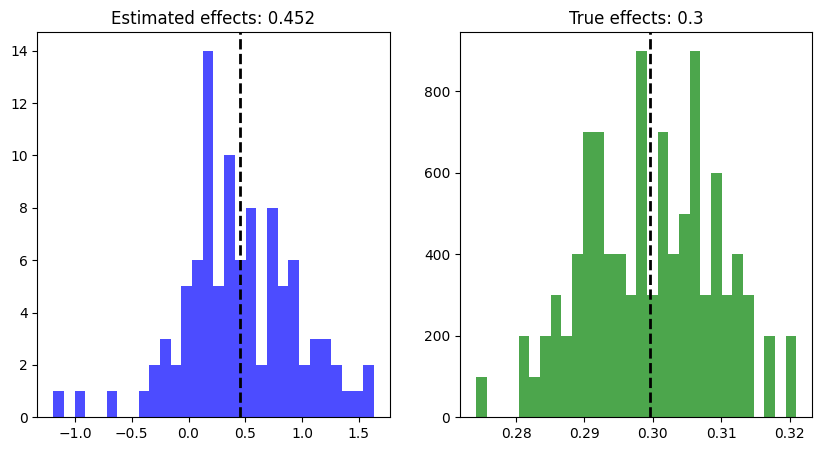
\includegraphics[width=0.8\textwidth]{fig_thesis.png} 
    \caption{Distribution of average estimated and true effects.}
    \label{fig:effects_distribution}
\end{figure}


\section{Discussion}
One limitation of this study is that it relies on synthetic data and idealized network structures, such as the adjacency matrix, which may not accurately reflect the complexity of real-world networks. In real-world scenarios, network structures are often dynamic, and detailed information about the connections between units may not be available. The study also focuses on the effects of network interference within static networks and does not account for evolving interactions or complex contagion. This shows the limits of applications of the provided adjustment method.  

To address these limitations and enhance the applicability of the findings, future research will focus on several key directions. First, we will explore nonrandom assignment mechanisms to better reflect real-world settings where treatment assignment is often influenced by underlying network characteristics or external factors. Second, advanced representation learning techniques, such as Node2Vec, will be integrated to better capture node representations. These extensions will enable a deeper understanding of the estimations under network interference in complex networks.

\bibliography{lit.bib}

\end{document}
